\def\QRCODE{TB_IPR_TUT.IMG.boolean_models_matlabqrcode.png}
\def\QRPAGE{http://www.iptutorials.science/tree/master/TB_IPR/TUT.IMG.boolean_models/matlab}
\mcorrectionsection{Matlab correction}

%\begin{mcomment}
%\begin{mremark}
%Please notice that when using boolean arrays in matlab, the notations $1-X$ and $\sim X$ are equivalent. When using uint8 arrays, verify that the values range into [0;1].
%\end{mremark}
%\end{mcomment}

\subsection{Simulation of a 2-D Boolean model}
The process for simulating the proposed Boolean model of 2-D disks consists in four steps:
\begin{itemize}
\item Generate the random number of points (by using the intensity parameter of the Poisson distribution). 
In order to avoid edge effects, one consider a larger window than the observation window to generate the disks.
Indeed, a germ outside the observation window can generate a disk that intersects the observation window. 
\item Generate the random locations of the germs (random coordinates from a uniform distribution)
\item Generate the random size of the disks (random radius from a probability distribution)
\item Generate the union of disks (by using the dilation of the germs with a disk of the corresponding radius as structuring element)
\end{itemize}

Here is the global function for generating such a Boolean model as a binary image:
\begin{matlab}
function Z = BooleanModel(Wsize, Gamma, RadiusParam)
% Generates a boolean model of disks in 2D. The number of disks is chosen according to a Poisson law of parameter lambda = Gamma*areaW, where areaW is the area of the window defined by Wsize.
%
% Wsize: size of the window (2x1 array)
% Gamma: Parameter to get the density for the Poisson law
% RadiusParam: [min, max] valus of radii
% returns: boolean array of size Wsize(1)xWsize(2)

edgeEffect = 2*max(RadiusParam)+100;
WsizeExtended = [Wsize(1)+2*edgeEffect,Wsize(2)+2*edgeEffect];
% nb of points
nf = WsizeExtended(1);
nc = WsizeExtended(2);
areaW = nf*nc;
nbPoints = poissrnd(Gamma*areaW);
% germs
x = randi(nf, nbPoints);
y = randi(nc, nbPoints); 
% grains
r = randi(RadiusParam, nbPoints);
Z = false(nf,nc);

% union of grains
[X, Y] = meshgrid(1:nf, 1:nc);
for i = 1:nbPoints
    Z = Z | ((X-x(i)).^2+(Y-y(i)).^2)<= r(i)^2;
end
Z = Z(edgeEffect+1:edgeEffect+Wsize(1),edgeEffect+1:edgeEffect+Wsize(2));
\end{matlab}

When executing this function with the following parameters:
\begin{matlab}
% parameters
Wsize = [500 500];
Gamma = 100/Wsize(1)/Wsize(2);
RadiusParam = [10 30]; % uniform law between 20 and 50

% generation
Z = BooleanModel(Wsize,Gamma,RadiusParam);

% visualization
imshow(Z);
\end{matlab}
We get a realization of this Boolean model as a binary image in Fig.\ref{fig:boolean_models:matlab:bmdisks}.
\begin{figure}[h]
\centering
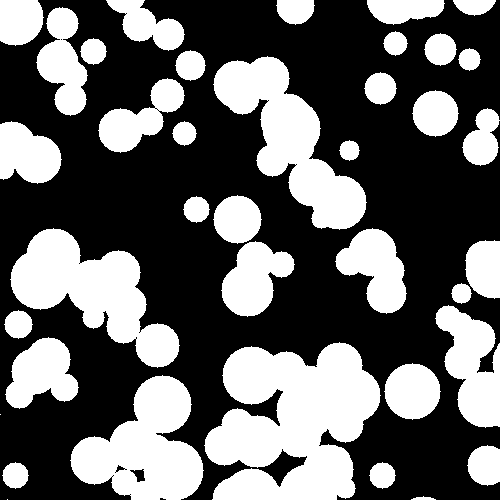
\includegraphics[width=.5\linewidth]{BMdisks}
\caption{Boolean model of disks, with $Wsize=[500,500]$ and $RadiusParam=[10,30]$.}
\label{fig:boolean_models:matlab:bmdisks}
\end{figure}


\subsection{Geometrical characterization of a 2-D Boolean model}
We can use the following function to compute the Minkowski functionals of the Boolean model (see the tutorial on Integral Geometry):
\begin{matlab}
function [Area, Perimeter, EulerNb4, EulerNb8] = MinkowskiFunctionals(X)

% Neighborhood configuration
F = [0 0 0; 0 1 4; 0 2 8];
XF = conv2(double(X),F,'same');
h = hist(XF(:),16);
%bar(0:15,h);

% Computation of the functionals
f_intra = [0 1 0 1 0 1 0 1 0 1 0 1 0 1 0 1];
e_intra = [0 2 1 2 1 2 2 2 0 2 1 2 1 2 2 2];
v_intra = [0 1 1 1 1 1 1 1 1 1 1 1 1 1 1 1];
EulerNb8 = sum(h.*v_intra - h.*e_intra + h.*f_intra);
f_inter = [0 0 0 0 0 0 0 0 0 0 0 0 0 0 0 1];
e_inter = [0 0 0 1 0 1 0 2 0 0 0 1 0 1 0 2];
v_inter = [0 1 0 1 0 1 0 1 0 1 0 1 0 1 0 1];
EulerNb4 = sum(h.*v_inter - h.*e_inter + h.*f_inter);
Area = sum(h.*f_intra);
Perimeter = sum(-4*h.*f_intra + 2*h.*e_intra);
\end{matlab}

So we can estimate the Minkowski densites on different realizations of  the Boolean model:
\begin{matlab}
% use of the Tutorial "Integral Geometry"
% computation of the Minkowski densities on different realizations
nbRealizations = 100;
W = zeros(nbRealizations,3);
areaWsize = Wsize(1)*Wsize(2);
for i = 1:nbRealizations
    [Z] = BooleanModel(Wsize,Gamma,RadiusParam);
    [area, per, ~, chi8] = MinkowskiFunctionals(Z);
    W(i,:) = [area, per/2, chi8*pi]/areaWsize;
    clear area per chi4 chi8;
end
\end{matlab}

Therefater, we can compare the estimated Minkowski mean densities of the Boolean model with the theoretical ones (by using the known parameters of the different probability distributions of this Boolean model):

\begin{matlab}
% mean densisties (estimated)
W = mean(W,1);

% mean densities (theoretical) by using Miles formulas
rMean = (RadiusParam(1)+RadiusParam(2))/2;
AreaMean = pi*rMean^2;
PerMean = 2*pi*rMean;
W_X = Gamma * [AreaMean,PerMean/2,pi];
W_th(1) = 1 - exp(-W_X(1));
W_th(2) = exp(-W_X(1)) * W_X(2);
W_th(3) = exp(-W_X(1)) * (W_X(3)-W_X(2)^2);

% comparison
error_W0 = abs(W(1)-W_th(1))/W_th(1)
error_W1 = abs(W(2)-W_th(2))/W_th(2)
error_W2 = abs(W(3)-W_th(3))/W_th(3)
\end{matlab}

\noindent Here are the results for 100 specific realizations:
\begin{mwindow}
errorW0 = 0.0701
errorW1 = 0.2437
errorW2 = 0.4396
\end{mwindow}

The errors can be large due to the biais estimation of the Minkowski densities within an observation window (specifically for the perimeter and the Euler number). But you can use unbiased estimators which can be found in the literature.

\noindent Note that the Miles formulas can be inverted to estimate the Minkowski functionals of the typocal grain from the Minkowski mean densities of the Boolean model.
